现在已经确定了工作项之间通信的基本构建块,可以描述如何在内核中表示工作组栅栏和本地内存。记住,工作项之间的通信需要工作组的概念,因此这些概念只能在ND-Range内核和分层内核中表示,而不包括在数据并行内核的执行模型中。\par

本章将以第4章中介绍的矩阵乘法内核示例为基础,通过介绍执行矩阵乘法的工作组中工作项之间的通信。在许多设备上——但不一定是所有设备!——通过本地内存通信提高矩阵乘法内核的性能。\par

\begin{tcolorbox}[colback=blue!5!white,colframe=blue!75!black, title=关于矩阵乘法的注意事项]
本书中,矩阵乘法内核用于演示内核中的变化如何影响性能。尽管使用本章的技术可以在某些设备上提高矩阵乘法的性能,但矩阵乘法是非常常见的操作,以至于许多供应商已经实现了矩阵乘法的高度优化版本。厂商投入大量的时间和精力来实现和验证特定设备的功能,并且在某些情况下使用在标准并行内核中难以或不可能使用的功能或技术。
\end{tcolorbox}

\begin{tcolorbox}[colback=blue!5!white,colframe=blue!75!black, title=USE VENDOR-PROVIDED LIBRARIES!]
当供应商提供函数的库实现时,使用它而不是将函数重新实现!对于矩阵乘法,我们可以将oneMKL作为DPC++开发者英特尔oneAPI解决方案工具包的一部分。
\end{tcolorbox}

图9-4展示了我们第4章的矩阵乘法内核代码。\par

\hspace*{\fill} \par %插入空行
图9-4 第4章中的矩阵乘法内核
\begin{lstlisting}[caption={}]
h.parallel_for(range{M, N}, [=](id<2> id) {
	int m = id[0];
	int n = id[1];
	
	T sum = 0;
	for (int k = 0; k < K; k++)
		sum += matrixA[m][k] * matrixB[k][n];
		
	matrixC[m][n] = sum;
});
\end{lstlisting}

第4章中,我们注意到矩阵乘法算法具有高度的重用性,并且对工作项进行分组可以改善访问的局部性,从而提高缓存命中率。本章中,我们修改后的矩阵乘法内核将使用本地内存作为缓存,以保证访问的局部性,而不是依赖隐式缓存行为来提高性能。\par

\begin{tcolorbox}[colback=red!5!white,colframe=red!75!black]
对于许多算法来说,可以将本地内存看作显式缓存。
\end{tcolorbox}

图9-5是第4章修改后的代码,展示了一个由单行组成的工作组,这使得使用本地内存的算法更容易理解。注意,对于结果矩阵一行中的元素,每个结果元素都是使用来自一个输入矩阵的数据列计算,用蓝色和橙色显示。因为这个输入矩阵没有数据共享,所以不是理想的本地内存候选。但是,该行中的每个结果元素都访问另一个输入矩阵(绿色部分)中的完全相同的数据。由于此数据是重用的,因此它是可以作为工作组本地内存中获益的最佳候选。\par

\hspace*{\fill} \par %插入空行
图9-5 矩阵乘法中工作组和工作项的映射
\begin{center}
	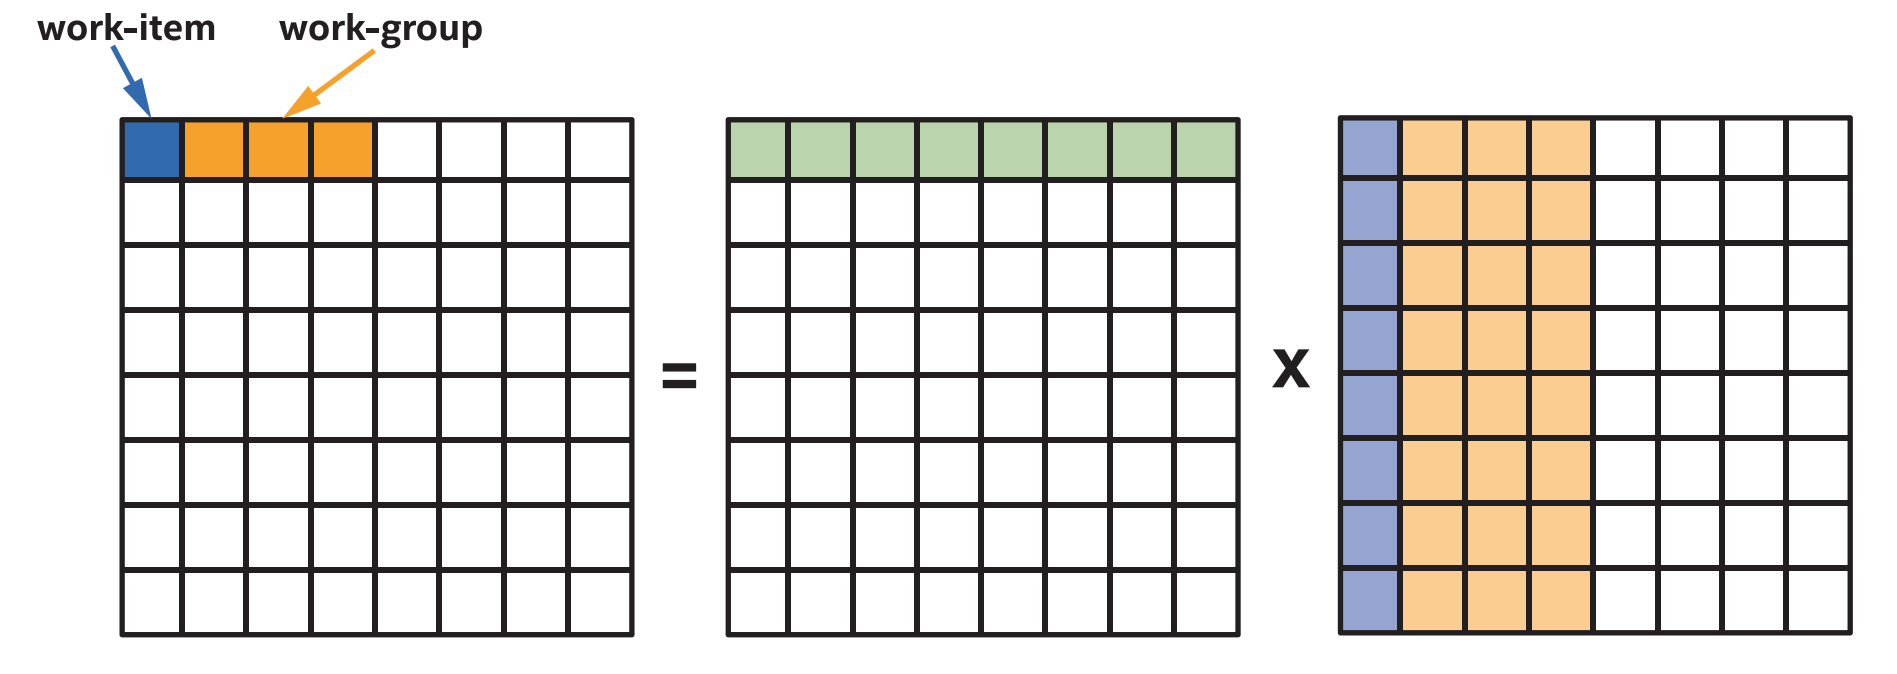
\includegraphics[width=1.\textwidth]{content/chapter-9/images/5}
\end{center}

因为要将非常大的矩阵相乘,而且工作组本地内存可能是有限的资源,所以我们修改后的内核将处理每个矩阵的子部分,将其称为矩阵块。对于每个块,我们修改后的内核将把矩阵块的数据加载到本地内存中,同步组中的工作项,然后从本地内存而不是全局内存加载数据。第一个块所访问的数据如图9-6所示。\par

内核中选择了与工作组大小相等的块大小。这不是必需的,但是因为它简化了本地内存的数据传输,所以块的大小通常可以选择工作组大小的倍数。\par

\hspace*{\fill} \par %插入空行
图9-6 处理第一个块:绿色的输入数据(X的左边)重用并从本地内存读取,蓝色和橙色的输入数据(X的右边)从全局内存读取
\begin{center}
	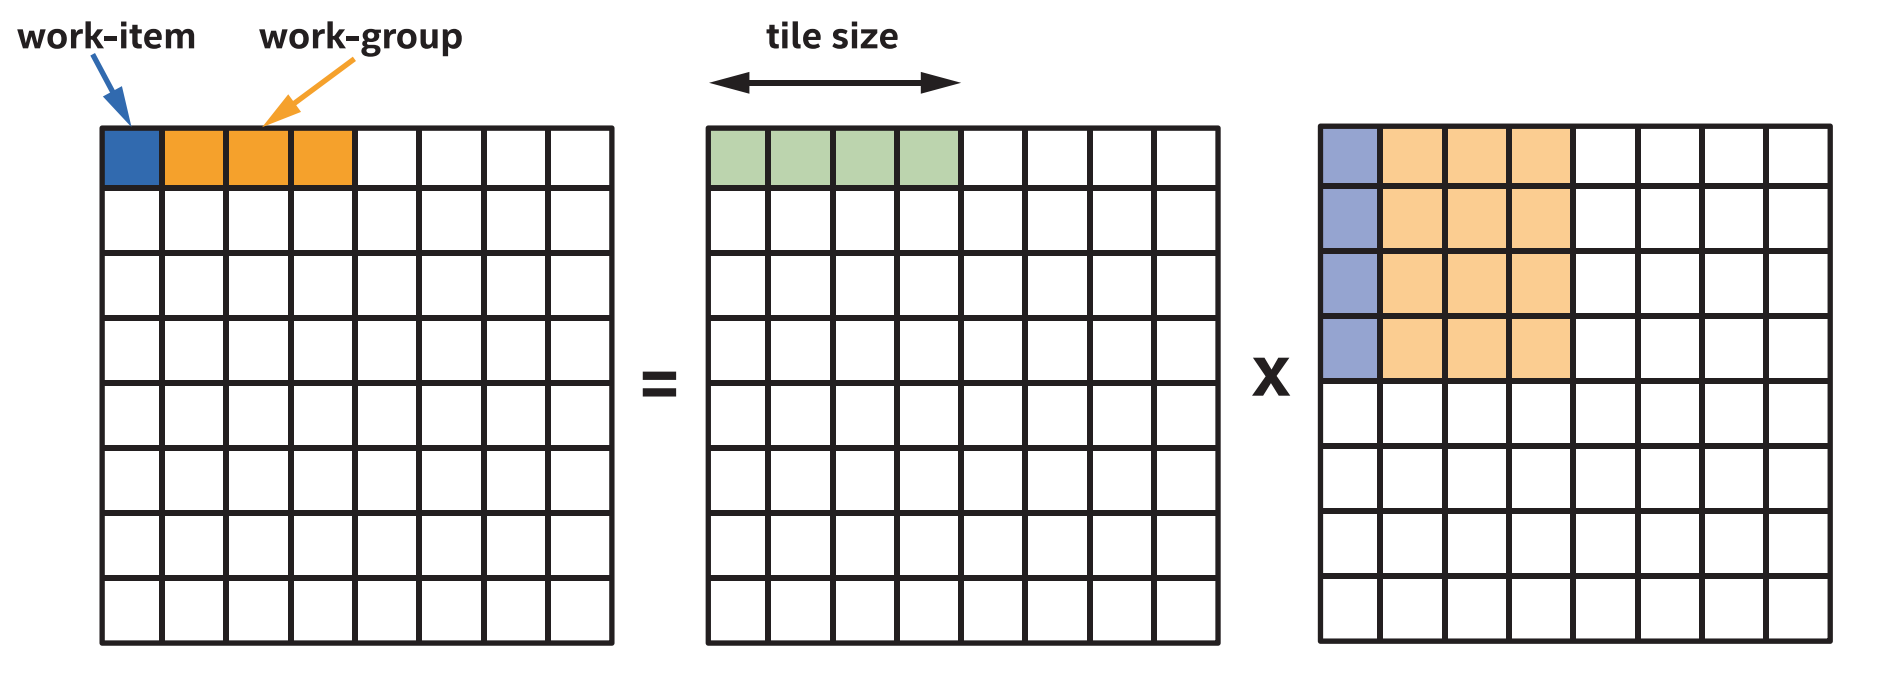
\includegraphics[width=1.\textwidth]{content/chapter-9/images/6}
\end{center}

\hspace*{\fill} \par %插入空行
\textbf{ND-Range内核中的工作组栅栏和本地内存}

本节描述如何在ND-Range内核中表示工作组栅栏和本地内存。对于ND-Range内核,是显式表示的:内核声明并操作本地地址空间分配的本地访问器,调用栅栏函数来同步工作组中的工作项。\par

\hspace*{\fill} \par %插入空行
\textbf{本地内存访问器}

要声明在ND-Range内核中使用的本地内存,请使用本地访问器。与其他访问器对象一样,本地访问器在命令组处理程序中构造,但与第3章和第7章讨论的访问器对象不同,本地访问器不是从缓冲区对象创建的。相反,通过指定类型和描述该类型元素数量的范围来创建局部访问器。与其他访问器一样,本地访问器可以是1维、2维或3维的。图9-7演示了如何声明本地访问器并在内核中使用。\par

请记住,本地内存在每个工作组开始时未初始化,每个工作组完成后不会持续保存数据。这意味着本地访问器必须是read\_write,否则内核将无法分配本地内存的内容或查看分配的结果。但是,本地访问器可以选择为原子的,这种情况下,通过访问器对本地内存的访问是原子执行的。原子访问将在第19章进行更详细的讨论。\par

\hspace*{\fill} \par %插入空行
图9-7 声明和使用本地访问器
\begin{lstlisting}[caption={}]
// This is a typical global accessor.
accessor dataAcc {dataBuf, h};

// This is a 1D local accessor consisting of 16 ints:
local_accessor<int> localIntAcc{16, h};

// This is a 2D local accessor consisting of 4 x 4 floats:
local_accessor<float,2> localFloatAcc{{4,4}, h};

h.parallel_for(nd_range<1>{{size}, {16}}, [=](nd_item<1> item) {
	auto index = item.get_global_id();
	auto local_index = item.get_local_id();
	
	// Within a kernel, a local accessor may be read from
	// and written to like any other accessor.
	localIntAcc[local_index] = dataAcc[index] + 1;
	dataAcc[index] = localIntAcc[local_index];
});
\end{lstlisting}

\hspace*{\fill} \par %插入空行
\textbf{同步功能}

同步ND-Range内核工作组中的工作项,请调用nd\_item类中的barrier函数。因为barrier函数是nd\_item类的成员,所以它只对ND-Range的内核可用,而对简单的数据并行内核或分层内核不可用。\par

barrier函数目前接受一个参数来描述要同步的内存空间,但是barrier函数的参数将来可能会随着SYCL和DPC++中内存模型的发展而改变。但是,barrier函数的参数提供了关于同步内存空间或内存同步域的控制。\par

当没有参数传递给barrier函数时,barrier函数将使用功能上正确和默认值。本章中的代码示例使用这种方式,以获得最大的可移植性和可读性。对于高度优化的内核,建议精确地描述哪些内存空间或哪些工作项必须同步,这可能会提高性能。\par

\hspace*{\fill} \par %插入空行
\textbf{一个完整的ND-Range内核示例}

现在知道了如何声明本地内存访问器并使用barrier函数同步对它的访问,我们可以实现矩阵乘法的ND-Range内核版本,协调工作组中工作项之间的通信,以减少对全局内存的通信。完整示例如图9-8所示。\par

\hspace*{\fill} \par %插入空行
图9-8 用ND-range parallel\_for和工作组本地内存表示块矩阵乘法内核
\begin{lstlisting}[caption={}]
// Traditional accessors, representing matrices in global memory:
accessor matrixA{bufA, h};
accessor matrixB{bufB, h};
accessor matrixC{bufC, h};

// Local accessor, for one matrix tile:
constexpr int tile_size = 16;
local_accessor<int> tileA{tile_size, h};

h.parallel_for(
nd_range<2>{{M, N}, {1, tile_size}}, [=](nd_item<2> item) {
	// Indices in the global index space:
	int m = item.get_global_id()[0];
	int n = item.get_global_id()[1];
	
	// Index in the local index space:
	int i = item.get_local_id()[1];
	
	T sum = 0;
	for (int kk = 0; kk < K; kk += tile_size) {
		// Load the matrix tile from matrix A, and synchronize
		// to ensure all work-items have a consistent view
		// of the matrix tile in local memory.
		tileA[i] = matrixA[m][kk + i];
		item.barrier();
		
		// Perform computation using the local memory tile, and
		// matrix B in global memory.
		for (int k = 0; k < tile_size; k++)
			sum += tileA[k] * matrixB[kk + k][n];
		
		// After computation, synchronize again, to ensure all
		// reads from the local memory tile are complete.
		item.barrier();
	}

	// Write the final result to global memory.
	matrixC[m][n] = sum;
});
\end{lstlisting}

这个内核中的主循环可以看作两个不同的阶段:第一个阶段,工作组中的工作项将共享数据从A矩阵加载到工作组本地内存中;第二种情况下,工作项使用共享的数据执行自己的计算。为了确保所有工作项在进入第二个阶段之前已经完成了第一阶段,两个阶段通过调用barrier来同步所有工作项,并提供一个内存栅栏来分隔。这种模式很常见,内核中使用工作组本地内存总是需要使用工作组栅栏。\par

注意,还必须调用barrier来同步当前块的计算阶段和下一个矩阵块的加载阶段之间的操作。如果没有此同步操作,则在用另一个工作项完成计算之前,工作组中的一个工作项可能会覆盖当前矩阵块的一部分。通常,当一个工作项在本地内存中读写由另一个工作项读写的数据时,就需要同步。图9-8中,同步是在循环结束时完成的,但是在每个循环开始时同步也是正确的。\par

\hspace*{\fill} \par %插入空行
\textbf{分层内核中的工作组栅栏和本地内存}

本节描述如何在分层内核中表示工作组栅栏和本地内存。与ND-Range内核不同,分层内核中的本地内存和栅栏是隐式的,不需要特殊的语法或函数调用。一些开发者会发现分层内核表示更直观、更容易使用,而其他开发者会喜欢ND-Range内核提供的直接控制。大多数情况下,相同的算法可能使用两种表示来描述,因此可以选择最容易开发和维护的方式。\par

\hspace*{\fill} \par %插入空行
\textbf{本地内存和栅栏的作用域}

回顾第4章,分层内核通过使用parallel\_for\_work\_group和parallel\_for\_work\_item函数来表示两级的并行执行。并行执行的这两个级别(或作用域)用于表示变量是否位于工作组本地内存中,并在工作组中的所有工作项之间共享,或者变量是否位于每个工作项私有内存中(不在工作项之间共享)。这两个作用域还用于同步工作组中的工作项,并强制执行内存一致性。\par

图9-9展示了一个示例层次结构内核,在本地内存中声明一个在工作组作用域的变量,加载到其中,然后在工作项作用域中使用该变量。在工作组作用域对本地内存的写入和工作项作用域对本地内存的读取之间存在一个隐式的栅栏。\par

\hspace*{\fill} \par %插入空行
图9-9 具有局部内存变量的分层内核
\begin{lstlisting}[caption={}]
range group_size{16};
range num_groups = size / group_size;

h.parallel_for_work_group(num_groups, group_size, [=](group<1> group) {
	// This variable is declared at work-group scope, so
	// it is allocated in local memory and accessible to
	// all work-items.
	int localIntArr[16];
	
	// There is an implicit barrier between code and variables
	// declared at work-group scope and the code and variables
	// at work-item scope.
	
	group.parallel_for_work_item([&](h_item<1> item) {
		auto index = item.get_global_id();
		auto local_index = item.get_local_id();
		
		// The code at work-item scope can read and write the
		// variables declared at work-group scope.
		localIntArr[local_index] = index + 1;
		data_acc[index] = localIntArr[local_index];
	});
});
\end{lstlisting}

分层内核表示的主要优点是,看起来非常类似于标准C++代码,标准C++代码中,一些变量可以在作用域中赋值,并在嵌套作用域中使用。当然,这也可以认为是一种缺点,因为哪些变量在本地内存中,以及什么时候必须由分层内核编译器插入栅栏,这些都不是很明显。对于实现栅栏非常昂贵的设备来说尤其如此!\par

\hspace*{\fill} \par %插入空行
\textbf{一个完整的分层内核示例}

既然知道了如何在分层内核中表示本地内存和栅栏,就可以编写一个分层内核,可以实现与图9-7中的ND-Range内核相同的算法,如图9-10所示。\par

尽管分层内核与ND-Range内核非常相似,但有一个关键的区别:在ND-Range内核中,矩阵乘法的结果在写入到内存中的输出矩阵之前累积到每个工作项变量和中,而分层内核则累积到内存中。也可以在分层内核中积累为每个工作项变量,但这需要特殊的private\_memory语法在工作组作用域声明每个工作项数据,而选择使用分层内核语法的原因之一是避免使用特殊语法!\par

\begin{tcolorbox}[colback=red!5!white,colframe=red!75!black]
分层内核不需要特殊的语法来声明工作组本地内存中的变量,但是需要特殊的语法来声明工作项私有内存中的一些变量!
\end{tcolorbox}

为了避免每个工作项的特殊数据语法,层次化内核中工作项循环的常见模式是将中间结果写入工作组本地内存或全局内存。\par

\hspace*{\fill} \par %插入空行
图9-10 块矩阵乘法内核作为层次内核实现
\begin{lstlisting}[caption={}]
const int tileSize = 16;
range group_size{1, tileSize};
range num_groups{M, N / tileSize};

h.parallel_for_work_group(num_groups, group_size, [=](group<2> group) {
	// Because this array is declared at work-group scope
	// it is in local memory
	T tileA[16];
	
	for (int kk = 0; kk < K; kk += tileSize) {
		// A barrier may be inserted between scopes here
		// automatically, unless the compiler can prove it is
		// not required
		
		// Load the matrix tile from matrix A
		group.parallel_for_work_item([&](h_item<2> item) {
			int m = item.get_global_id()[0];
			int i = item.get_local_id()[1];
			tileA[i] = matrixA[m][kk + i];
		});
	
		// A barrier gets inserted here automatically, so all
		// work items have a consistent view of memory
		
		group.parallel_for_work_item([&](h_item<2> item) {
			int m = item.get_global_id()[0];
			int n = item.get_global_id()[1];
			for (int k = 0; k < tileSize; k++)
			matrixC[m][n] += tileA[k] * matrixB[kk + k][n];
		});
	
		// A barrier gets inserted here automatically, too
	}
});
\end{lstlisting}

图9-10中内核一个有趣的属性与循环迭代变量kk有关:由于循环处于工作组作用域,循环迭代变量kk可以从工作组本地内存中分配,就像tileA数组一样。在这种情况下,由于kk的值对于工作组中的所有工作项都是相同的,所以编译器可能会选择在每个工作项内存中分配kk,特别是对于本地内存稀缺的设备。\par























